\section{Definizione}
Il ciclo di vita del software definisce un modello per il software, dalla sua concezione iniziale fino al suo sviluppo completo, al suo rilascio, alla sua successiva evoluzione, fino al suo ritiro. \\
Un \textit{software cycle} suddivide quindi l'attività di realizzazione di prodotti software in sottoattività fra loro coordinate, il cui risultato finale è il prodotto stesso e tutta la documentazione ad esso associata. Fasi tipiche includono lo studio o analisi, la progettazione, la realizzazione, il collaudo, la messa a punto, la manutenzione e l'estensione.

\section{Un modello a cascata}
Definiamo di seguito i principali punti in cui si tende a suddividere lo sviluppo di un software.
\begin{enumerate}
	\item \textbf{Studio di fattibilità e controllo dei requisiti}
		\begin{itemize}
			\item Valutare costi e benefici
			\item Pianificare attività e risorse di progetto
			\item Individuare ambiente di programmazione (hardware/software)
			\item Raccogliere i requisiti
		\end{itemize}
	\item \textbf{Analisi dei requisiti} \hfill \\
		Gli analisti informatici hanno il compito di descrivere il dominio di applicazione e specificare varie componenti nello \textit{schema concettuale}
		\footnote{\textbf{Schema concettuale:} Insieme di documenti che definiscono in termini \textit{concettuali}, in modo logico/matematico, tutti gli elementi del software. 
		Include l'analisi dei dati, le funzionalità finali del software e tutte le componenti richieste.}.
	\item \textbf{Progetto e realizzazione} \hfill \\
		I progettisti descrivono la realizzazione del software a partire dal suo schema concettuale.
		\begin{itemize}
			\item Architettura del programma
			\item Struttura di realizzazione
			\item Scrittura del codice e documentazione
		\end{itemize}
	\item \textbf{Verifica} \hfill \\
		Nel verificare la correttezza e la completezza del software vengono spesso utilizzati strumenti matematici e logici	per \textit{dimostrare} il funzionamento del programma sul modello del software (non sul software stesso).
	\item \textbf{Manutenzione}
		\begin{itemize}
			\item Controllo durante l'esercizio del programma
			\item Eventuali correzioni/aggiornamenti del programma
		\end{itemize}
\end{enumerate}
Quello appena descritto è un tipico \textit{ciclo a cascata}, nel quale ogni 'step' viene eseguito interamente una volta sola e termina con il rilascio finale dell'applicativo.\\
Tale modello non è funzionale.\\
Si pensi, ad esempio, al ruolo dei programmatori: all'interno di un ciclo di vita del software come quello sopra, già dal primo punto si suppone di aver assunto un team di sviluppatori che non inizieranno a lavorare prima della fine del punto 3 - a mesi di distanza dall'assunzione. Anche escludendo i costi di mantenimento di un team (che per giunta non lavora), appare chiaro come questo ciclo richieda fin troppo tempo e spreco di risorse.\\
Cosa accadrebbe, inoltre, se alla consegna del progetto il cliente non fosse soddisfatto?

\section{Un modello a spirale}
Per i motivi visti nella sezione precedente, si considera più ottimizzato e funzionale un ciclo di vita \textit{a spirale}:

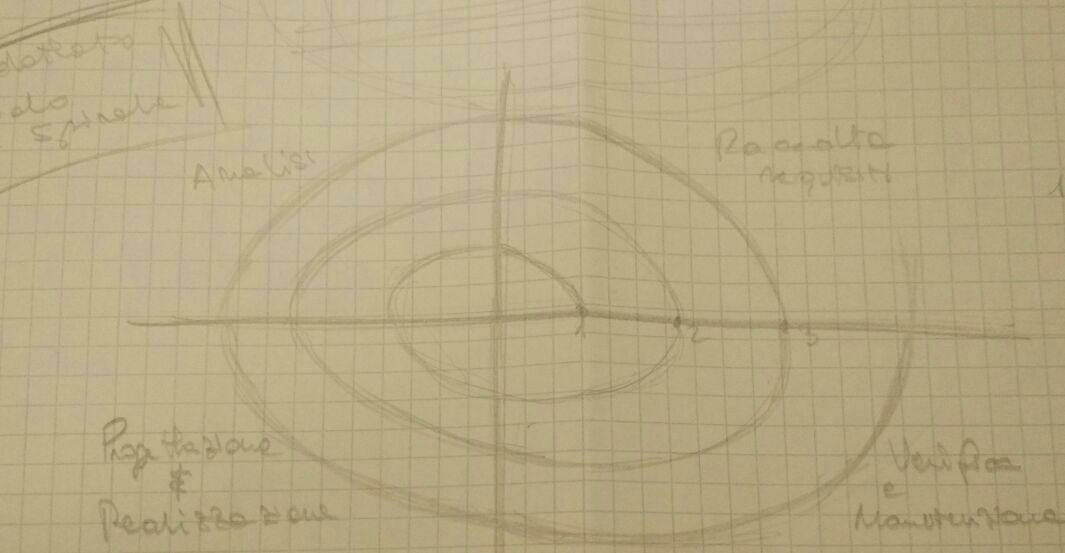
\includegraphics[width=\textwidth]{spiral.jpg} \hfill \\ \\
Partendo dal centro, si inizia un ciclo seguendo un modello come quello descritto nella sezione precedente; alla fine del primo 'ciclo' della spirale, dopo un tempo relativamente limitato (spesso circa 3 mesi), si rilascia \textit{una prima \textit{}versione} dell'applicazione.\\
Questa versione deve essere minimale ma funzionale - un software parziale ma già utilizzabile dall'utente finale, che nell'usarla darà istruzioni per la correzione e l'implementazione di funzioni. Ad ogni ciclo della spirale corrisponde quindi il rilascio di versioni via via più complete, fino ad arrivare al rilascio finale.

\subsection{La doppia spirale}
Il rischio di questo modello rimane, seppur in maniera di gran lunga ridotta, lo stesso del modello a cascata per quanto riguarda lo sfruttamento del tempo a disposizione. \\
Poichè di frequente è richiesto di ottimizzare il più possibile il tempo e le risorse di cui si dispone, non è raro l'utilizzo di un procedimento a \textit{doppia spirale}: alla consegna della prima raccolta di requisiti agli analisti, non appena si dispone di una previsione del tempo necessario per il rilascio della prima versione, si inizia una seconda raccolta di requisiti in previsione della seconda versione del software; in questo modo, quando gli sviluppatori inizieranno a scrivere la prima versione, i progettisti avranno già pronto lo schema per la progettazione della seconda versione. \\
Tra i vantaggi che porta l'utilizzo di questo metodo, oltre alla grande ottimizzazione del tempo, forse il più importante è che permette di apportare modifiche, correzioni e aggiunta di funzionalità al prodotto in maniera molto rapida grazie alla costante comunicazione con l'utente finale.